\chapter{Opis implementacji}
\label{cha:implementacja}

Zgodnie z opisanymi w poprzednim rozdziale pracy założeniami architektury dla proponowanych rozwiązań zaimplementowano przykładowe aplikacje prezentujące wykorzystanie koncepcji systemów zarządzania tożsamościami przy użyciu specyfikacji SAML. Najbardziej podstawowym spośród zrealizowanych scenariuszy było zastosowanie asercji SAML w procesie uwierzytelniania klientów aplikacji webowych - udostępnianych poprzez przeglądarkę internetową. Implementacja tego przypadku była punktem wyjścia dla wdrożenia koncepcji zarządzania tożsamościami dla systemów w architekturze zorientowanej na usługi. Opracowane zostały aplikacje wykorzystujące standard SAML w procesie uwierzytelniania klientów usług webowych(przy użyciu standardów SOAP i REST). Zaimplementowano usługi realizujące poszczególne etapy procesu dokonywania zamówienia w sklepie internetowym. Usługi zostały wykorzystane jako przykład zastosowania mechanizmów SAML w architekturze SOA. Wprowadzona została warstwa pośrednicząca pomiędzy wywołaniami klienta a dostarczanymi serwisami - magistrala usług ESB. Zastosowano również narzędzia modelowania procesów biznesowych w celu skomponowania procesu realizacji zamówienia przy użyciu dostępnych usług z wykorzystaniem uwierzytelniania opartego o tokeny bezpieczeństwa SAML. 

\section{Implementacja mechanizmu jednokrotnego uwierzytelniania klientów aplikacji webowych}

	Przy pomocy mechanizmów udostępnianych przez narzędzia \textit{Picketlink} zaimplementowana została usługa ,,Identity Provider'' odpowiedzialna za uwierzytelnianie użytkowników systemu. Stosując usługę IDP możliwe jest jednokrotne uwierzytelnianie klientów aplikacji webowych. Zaimplementowane zostały również aplikacje wykorzystujące usługę IDP jako mechanizm uwierzytelniania klientów żądających dostępu do zasobów aplikacji.

	\begin{figure}[h]
		\centering
		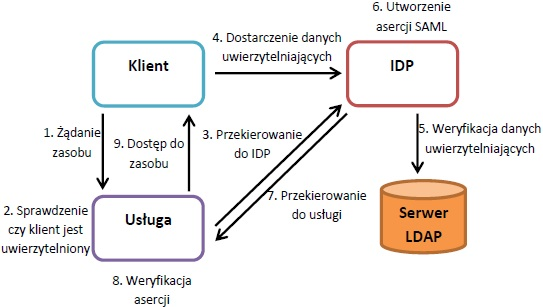
\includegraphics{img/samlWebSSO.jpg}
		\caption{Przebieg procesu jednokrotne uwierzytelnianie aplikacji webowych w protokole SAML}
		\label{samlSSOSteps}
	\end{figure}
		
	Kiedy użytkownik chce uzyskać dostęp do zasobów, usługa sprawdza czy klient jest uwierzytelniony. Jeśli nie jest uwierzytelniony następuje przekierowanie do usługi ,,Identity Provider''. Klient podaje swoje dane uwierzytelniające a IDP weryfikuje ich poprawność. Gdy dane są prawidłowe generowana jest asercja SAML i następuje przekierowanie do usługi. Usługa weryfikuje otrzymaną asercję i przydziela lub odmawia prawa dostępu do zasobu. Gdy klient chce uzyskać dostęp do zasobów innej aplikacji nie musi ponownie podawać swoich danych uwierzytelniających, usługa IDP nie dokonuje ponownie procesu uwierzytelniania w usłudze katalogowej LDAP.

\section{Implementacja modułu magistrali usług}

	Implementacja mechanizmu magistrali usług wykorzystuje framework ,,Switchyard''. Przy pomocy narzędzi ,,Switchyard'' konfigurowane są punkty końcowe, na których nasłuchiwane są nadchodzące komunikaty. Przetwarzanie otrzymanych wiadomości realizowane jest przy użyciu narzędzi ,,Camel''. ,,Camel'' dostarcza mechanizmy zarządzania ścieżką jaką kierowane są wiadomości  oraz implementuje wzorce EIP(\textit{Enterprise Integration Patterns}). Implementacja mechanizmu przetwarzania wiadomości magistrali usług przedstawiona zostanie na przykładzie wywołań serwisów webowych dostarczanych przy użyciu technologii SOAP(rysunek \textit{,,Implementacja przetwarzania wiadomości przez magistralę usług''}).

	\begin{figure}[h]
		\centering
		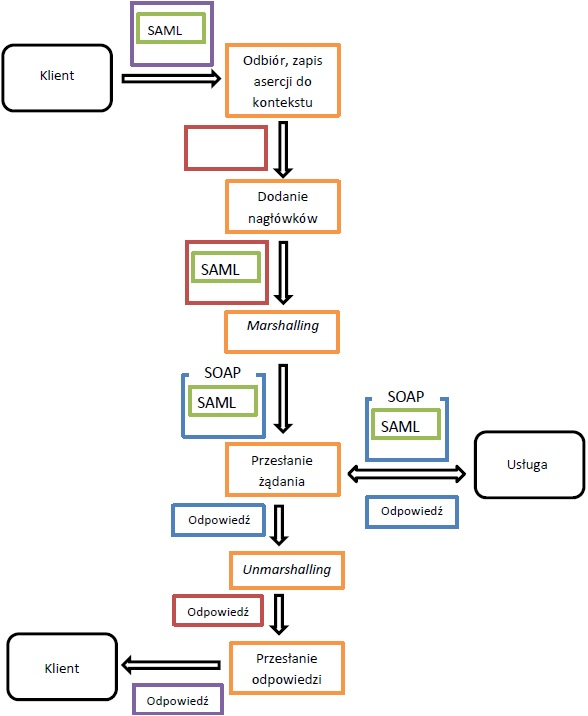
\includegraphics{img/esbRoute.jpg}
		\caption{Implementacja przetwarzania wiadomości przez magistralę usług}
		\label{ESB route}
	\end{figure}

	Klient wywołując usługi przesyła komunikaty określonego formatu - korzystając z określonej metody dostępu do zdalnych serwisów. Moduł magistrali usług otrzymuje komunikat żądania usługi. Do komunikatu dołączony jest nagłówek, w którym przesyłany jest token bezpieczeństwa - asercja SAML. Otrzymany komunikat przekształcany jest do formatu wykorzystywanego wewnętrznie przez moduł przetwarzania wiadomości a informacje zawarte w nagłówku(w tym asercja SAML) zapisywane są w kontekście przetwarzania. Do budowanej wiadomości dodawane są nagłówki(informacje kontekstowe) - dzięki czemu dołączany jest token bezpieczeństwa. Następnie dokonywany jest proces \textit{marshallowania} zbudowanej wiadomości - asercja SAML wpisywana jest do nagłówka(np. SOAP) utworzonego komunikatu. Po serializacji informacji następuje wywołanie usługi korzystające ze zbudowanej wiadomości. Usługa przeprowadza procesy uwierzytelniania klienta i autoryzacji dostępu do zasobów. Po poprawnym przebiegu tych kroków zwracana jest odpowiedź serwisu. Odpowiedź jest \textit{unmarshallowana} i przysłana do klienta w formacie zgodnym z metodą wywołania usługi.
	

%---------------------------------------------------------------------------
